\documentclass[12pt,letterpaper,twoside]{book}
\usepackage[utf8]{inputenc}
\usepackage[spanish]{babel}
\usepackage{amsmath}
\usepackage{amsfonts}
\usepackage{amssymb}
\usepackage{makeidx}
\usepackage{graphicx}
\usepackage{lmodern}
\usepackage{kpfonts}
\usepackage[left=2cm,right=2cm,top=2cm,bottom=2cm]{geometry}


\title{Microcontroladores de 32 bits}
\author{Dr. Casimiro Gómez González\\
	Facultad de Electrónica, UPAEP\\
               correo: casimiro.gomez@upaep.mx\\
               Tel: 222 229 9428}
\date{Primavera 2013}
\begin{document}
\frontmatter
\maketitle


\chapter{Prólogo}
El presente material ha sido desarrollado como parte del \textit{\textbf{Diplomado en Sistemas embebidos 
para Automatización y Robótica}} y es una recopilación de distintos materiales que se han ido desarrollando en el Laboratorio de Sistemas Embebidos (LSE) de la Universidad Popular Autónoma del Estado de Puebla (UPAEP) en México.
\begin{flushright}

El autor\\
Casimiro Gómez González\\
Doctor en Ingeniería Mecatrónica
\end{flushright}

\tableofcontents
\listoftables
\listoffigures

\mainmatter
\chapter{Introducción a Microprocesadores}
En este capítulo se describen las principales características de los microcontroladores de 32 bits.

\begin{figure}
\centering
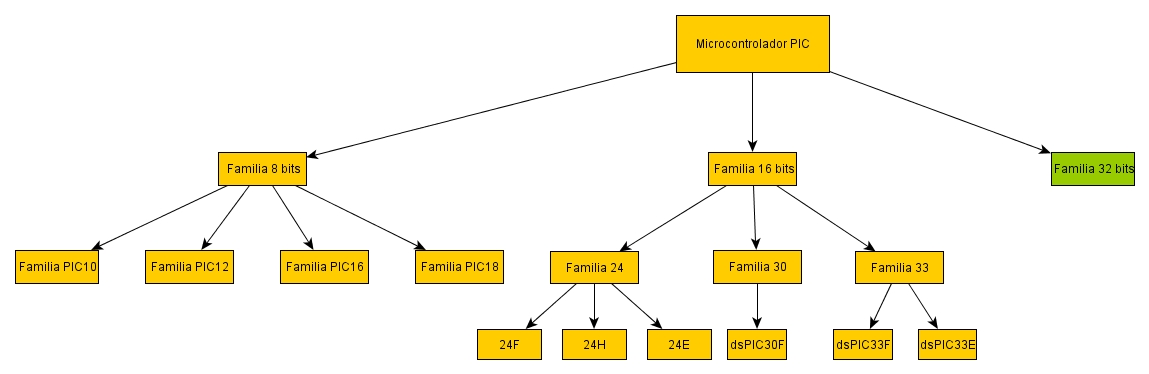
\includegraphics[width=6in]{Microchip.jpg}
\caption{Familias Microchip}
\label{fig0}
\end{figure}


\section{Descripción general}
La Familia de microcontroladores de 32 bits de Microchip (PIC32) cuenta con un funcionamiento más amplio y con una memoria de mayor capacidad, lo cual nos permite realizar diseños embebidos complejos.  Para  emplear  dichos micros, Microchip ofrece una plataforma de software gratuito conocido como MPLABX IDE, el cual usamos  a lo largo del curso.


\begin{figure}
\centering
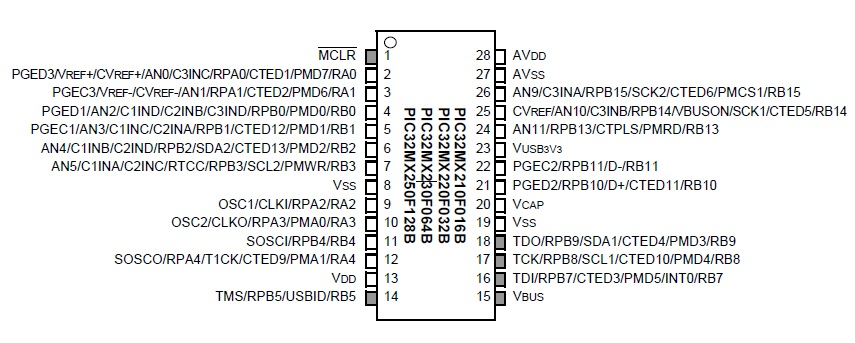
\includegraphics[width=4.5in]{32MX220F032B.jpg}
\caption{Pines del Microcontrolador 32MX220F032B}
\label{fig1}
\end{figure}

Para programar el PIC32MX220F032B utilizamos el PICkit 3, para ello  armamos un circuito para que el micro pueda ser reconocido por el Pickit3 y posteriormente grabarlo. El PICkit viene con un manual que muestra un diagrama de la forma de conectar el microprocesador. El pin uno de los PICkit está situado en el triángulo blanco. 

\begin{figure}
\centering
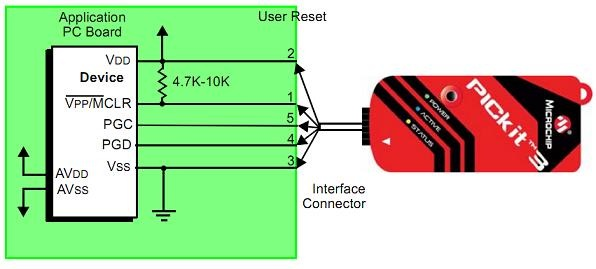
\includegraphics[width=5in]{Pickit3.jpg}
\caption{Conexión del PicKit3 para programar el Microcontrolador}
\label{fig2}
\end{figure}


\begin{figure}
\centering
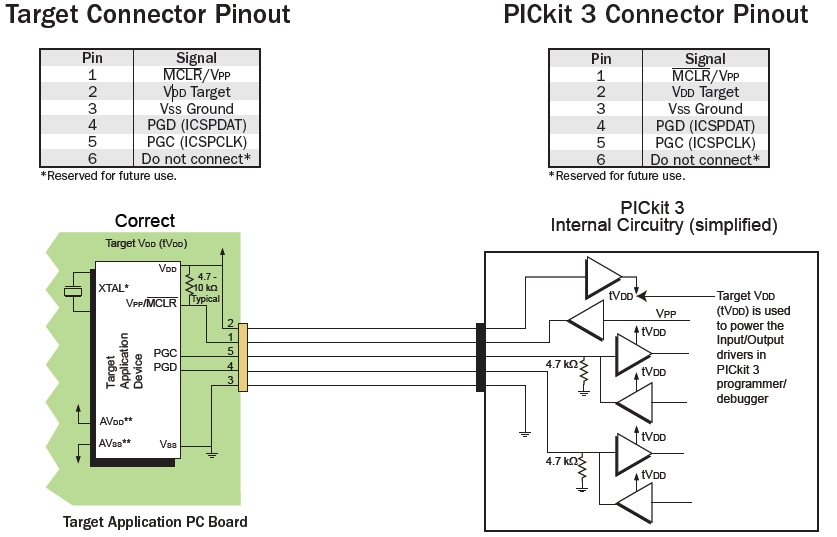
\includegraphics[width=5in]{conexionPickit3.jpg}
\caption{Conexión Interna del PicKit3 para programar el Microcontrolador}
\label{fig3}
\end{figure}

El PICkit tiene seis orificios en su extremo, cinco de ellos se encuentran conectados a  cinco pines correspondientes del microprocesador.
Sin embargo nos dimos cuenta que al conectar el PICkit 3 no identificaba el microprocesador, pues aparecía un error en MPLABX.IDE  a la hora de quemar el micro. Por ello decidimos adicionarle dos  capacitores de 0.1µf entre VDD y VSS para ayudar a estabilizar al sistema colocándolos muy cerca del PIC, y así purificar la señal.  

\begin{figure}
\centering
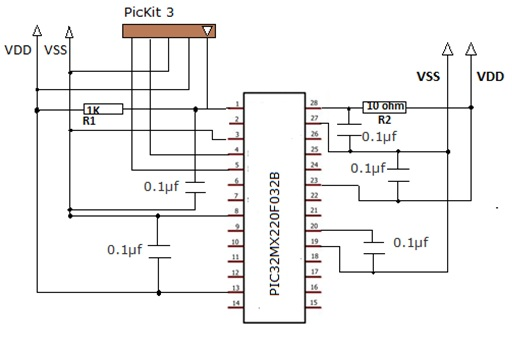
\includegraphics[width=5in]{Quemador.jpg}
\caption{Circuito para quemar PICs con el PicKit3}
\label{fig4}
\end{figure}

\section{Conexiones Mínimas}

Para utilizar el microcontrolador PIC32MX220F032B se requiere tener en cuenta las conexiones mínimas. A continuación se describe una lista de PINES, los cuales SIEMPRE deben estar conectados:

\begin{itemize}
\item Todos los pines $V_{dd}$ y $V_{ss}$
\item Todos los pines $AV_{ss}$ y $AV_{dd}$, aún y cuando el módulo del Convertidor Analógico Digital (CAD) no sea utilizado
\item EL pin $V_{CAP}$
\item EL pin $\overline{MCLR}$
\item Los pines OSC1 y OSC2 cuando se utiliza un oscilador externo.
\end{itemize}


\begin{figure}
\centering
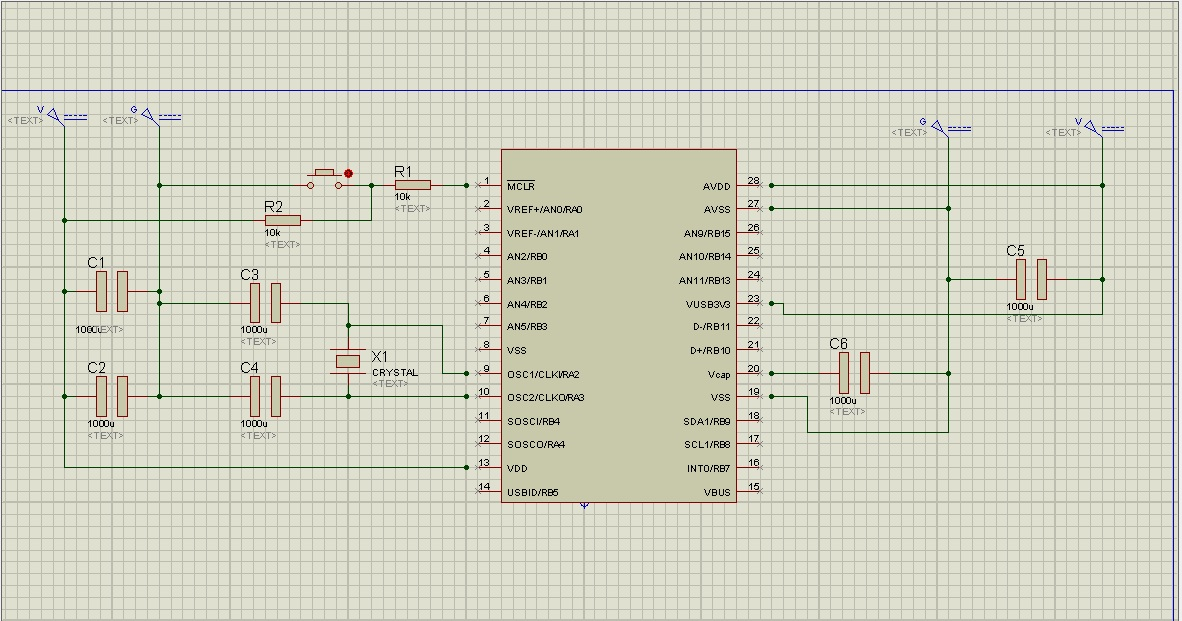
\includegraphics[width=5in]{conexionesminimas.jpg}
\caption{Conexiones Mínimas del 32MX220F032B}
\label{fig5}
\end{figure}


\section{Capacitores de desacoplo}

Para la correcta operación del Microcontrolador es necesario conectar capacitores de desacoplo en los pines de potencia, tales como, $V_{DD}$, $V_{SS}$, $AV_{DD}$ y $AV_{SS}$ como se muestra 

\begin{figure}
\centering
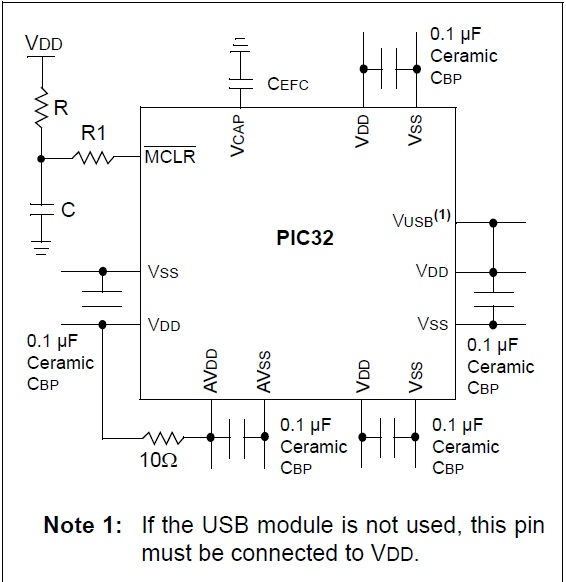
\includegraphics[width=5in]{capacitoresdesacoplo.jpg}
\caption{Capacitores de desacoplo}
\label{fig6}
\end{figure}

Cuando se utilizan capacitores de desacoplo deben considerarse los siguientes criterios:

\begin{itemize}
\item Valor y tipo de capacitor: Un valor de $0.1 \mu F$, $10-20V$ es recomendado. Se recomienda utilizar capacitores cerámicos 
\item Colocación en el PCB: Los capacitores de desacoplo deben colocarse tan cerca de los PINES del microcontrolador como sea posible. Se recomienda colocar los capacitores del mismo lado de la tarjeta de la que se encuentra el Microcontrolador. Si el espacio es limitado, el capacitor puede colocarse en otra capa del PCB usando una via, sin embargo, debemos asegurarnos que la distancia del pin al capacitor este en los $6mm$ de largo.
\item Manejando ruidos de Alta Frecuencia: Si la tarjeta experimenta ruido de alta frecuencia, arriba de $10 Mhz$, se tiene que adicionar un segundo capacitor ceramico en paralelo a los descritos en los capacitores de desacoplo. El valor de el segundo capacitor puede estar en el rango de $0.01 \mu F$ a $0.001 \mu F$. Se tiene que colar este segundo capacitor cerca del capacitor primario de desacoplo. Para el diseño de circuitos de alta frecuencia, se debe considerar instalar un par de capacitores tan cerca de los pines de potencia con diferencia de decadas, por ejemplo $0.1 \mu F$ en paralelo con $0.001 \mu F$. 
\end{itemize}

\begin{figure}
\centering
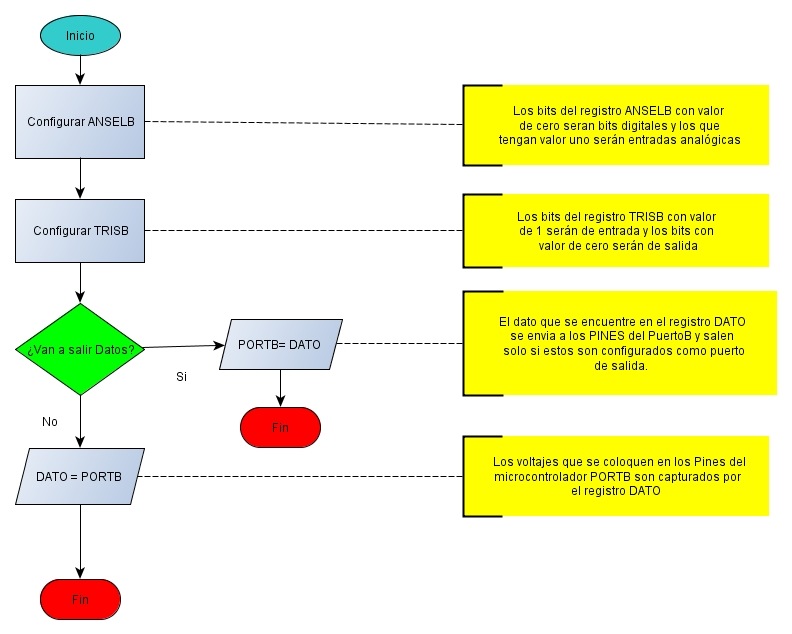
\includegraphics[width=5in]{ConfigurarPuertos.jpg}
\caption{Algoritmo para configurar Puertos}
\label{fig7}
\end{figure}

\subsection{Capacitores de Ruido de Fuente}

El uso de capacitores en la fuente de alimentación es recomendable para mejorar la estabilidad de la alimentación. Valores típicos en el rango de $4.7 \mu F$ a $47 \mu F$ son recomendables. Este capacitor debe estar localizado lo mas cerca posible del dispositivo.

\subsection{Capacitor del Regulador Interno de Voltaje ($V_{CAP}$)}

Un capacitor de bajo-ESR es necesario en el pin $V_{CAP}$, el cual es utilizado para estabilizar la salida el regulador interno. El pin $V_{CAP}$ no debe ser conectado a $V_{DD}$, y debe tener una capacitor $C_{EFC}$, con al menos $6V$ de voltaje, conectado a tierra. El tipo de capacitor es de cerámica o tantalio, con un valor en el rango de $8 \mu F$ a $10 \mu F$

\subsection{Pin \emph{Master Clear} $\overline{MCLR}$}

El Pin $\overline{MCLR}$ tiene dos funciones en el microcontrolador:
\begin{itemize}
\item Reset del Microcontrolador
\item Programación y depuración del microcontrolador
\end{itemize}

Conectando el Pin $\overline{MCLR}$ a tierra resetea el Microcontrolador. 


\begin{figure}
\centering
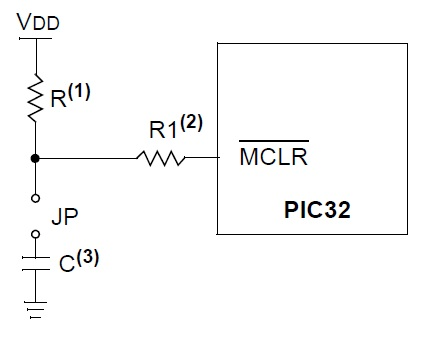
\includegraphics[width=3.5in]{reset.jpg}
\caption{Conexión del reset al microcontrolador}
\label{fig8}
\end{figure}

En la Figura \ref{fig8}, la resistencia $R1\leq 470 \Omega$  limitará cualquier corriente fluyendo a través del Pin $\overline{MCLR}$ desde el capacitor externo debido a descargas electrostáticas (ESD) o sobre estres eléctrico (EOS), asegurando que el pin $\overline{MCLR}$ alcanza las especificaciones de $V_{IH}$ y $V_{IL}$. La resistencia $R \leq 10 k \Omega $ es recomendad. Se recomiendan valores iniciales de $10 k \Omega$ para asegurar que el pin $\overline{MCLR}$ alcanza los valores $V_{IH}$ y $V_{IL}$ son alcanzados. El capacitor debe ser de tal tamaño que prevenga Resets accidentalmente debido a glitches o extender el reset del microcontrolador durante el periodo de $POR$.


\subsection{Pins sin utilizar}

Pins de I/O que esten sin se utilizados no deben de dejarse flotantes. Estos pueden ser configurados como salida y manejados a un valor lógico bajo.

Alternativamente, las entradas pueden reservarse conectando el pin a $V_{ss}$ a través de una resistencia de $1k$ a $10k$ y configurando el pin como entrada.

\section{El oscilador}

El sistema de oscilación del PIC32 tiene los siguientes módulos y características:

\begin{itemize}
\item Cuatro osciladores externos e internos como fuentes de reloj
\item Un PLL con un divisor y multiplicador, lo cual incrementa la frecuencia de operación ya sea de la fuente ineterna o externa
\item Un divisor postescalador integrado que selecciona la fuente de la cual proviene
\item Un interruptor seleccionable por sofware que eleige entre varias fuentes.
\item Un monitor de operación segura del reloj (FSCM) que detecta las fallas del reloj y permite a las aplicaciones recuperarse o apagarse.
\end{itemize}

La familia de dispositivos PIC32 tiene múltiples relojes internos que se derivan de las fuentes de reloj internas o externas. Algunas de estas fuentes de reloj tienen lazos de PLL (PLL), un divisor de salida programable, un divisor de entrada, para escalar de entrada de frecuencia y adaptarla a la aplicación. La fuente de reloj puede ser cambiada en ejecución por software. El registro de control del oscilador esta cerrado  por hardware, y y debe ser abierto por una serie de escrituras antes de que el reloj realice un cambio.

Hay tres relojes principales en los dispositivos PIC32:

\begin{itemize}
\item Reloj del Sistema (SYSCLK), usado en el CPU y algunos periféricos
\item Reloj del bus de periféricos (PBCLK) usado por la mayoria de periféricos
\item Reloj USB (USBCLK), usado por los periféricos USB
\end{itemize}

El reloj del PIC32 surgen de alguna de las siguientes fuentes:

\begin{itemize}
\item Oscilador Primario ($P_{OSC}$) en los pines OSC1 y OSC2
\item El oscilador secundario ($S_{OSC}$) en los pines SOSC1 y SOSC2
\item El oscilador rápido interno (FRC)
\item El oscilador de baja potencia (LPRC) 
\end{itemize}

Cada una de las fuentes de reloj tiene opciones de  configuración   únicas, tales como el PLL, el divisor de entrada y/o divisor de salida. 

\subsection{Generación de el reloj de sistema (SYSCLK)}

La señal SYSCLK es usado principalmente por el CPU y algunos periféricos tales como el DMA, el controlador de interrupciones y el cache de preFetch. La señal SYSCLK proviene de alguna de las cuatro fuentes de reloj:

\begin{itemize}
\item $P_{OSC}$
\item $S_{OSC}$
\item El oscilador interno rápido FRC
\item El oscilador LPRC
\end{itemize}


Algunas de las fuentes de reloj tienen opciones específicas de multiplicador y/o divisor. La fuente SYSCLK es seleccionada por la configuración del microcontrolador y puede cambiarse durante la operación por software. La habilidad para cambiar las fuentes de reloj durante la operación permite a la plicación reducir su cnsumo de potancia y reducir la velocidad de reloj.

\begin{figure}
\centering
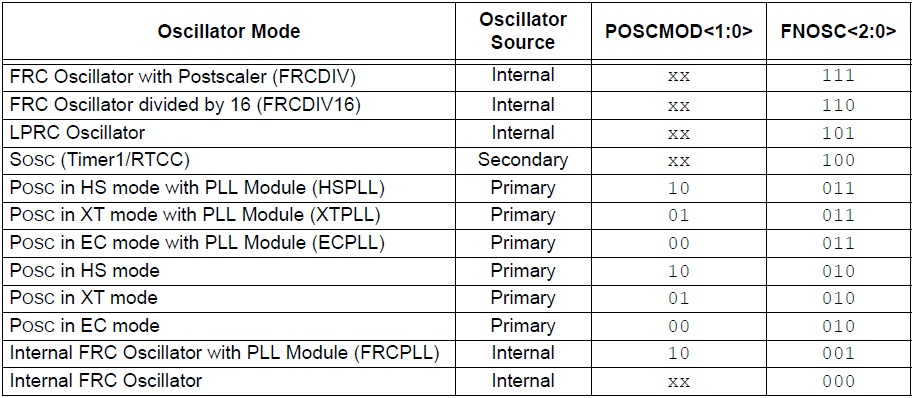
\includegraphics[width=4in]{oscilador.jpg}
\caption{Opciones del oscilador}
\label{fig9}
\end{figure}


\begin{figure}
\centering
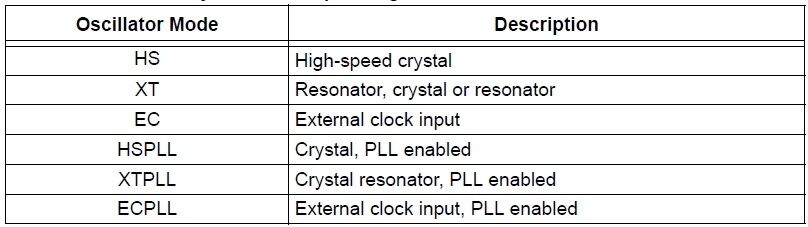
\includegraphics[width=4.5in]{osciladorPrimario.jpg}
\caption{Opciones del oscilador Primario}
\label{fig10}
\end{figure}

\begin{figure}
\centering
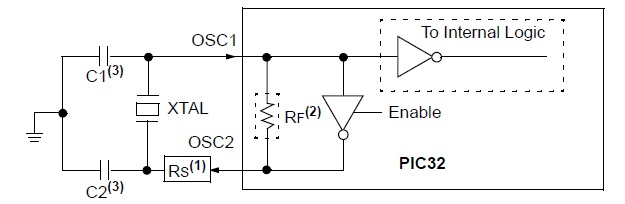
\includegraphics[width=4.5in]{cristal.jpg}
\caption{Conexiones del cristal}
\label{fig11}
\end{figure}


\bibliographystyle{alpha} %% plain.bst
\bibliography{./VerilogBibliografia}
\backmatter
\end{document}

